\subsubsection{Results Catalog Specifications}
The Results Catalog is where the user can view their already processed data stored in the backend. If this user is using a shared server, this can potentially also show processed data from \textit{other} users in their group, should those permissions be allowed.\par
The Results Catalog will be depicted in four separate parts, the first three of which involve searching, filtering and selecting specs, inputs, and jobs. While the last part revolves around viewing visualizations for the results of the selected jobs. It will usually be the case that users will create a large amount of jobs, corresponding to sets of sound files captured at various locations. Therefore, filtering jobs will be a necessary feature when selecting job results to analyze. The core functionality of the first part of the catalog is as follows:\\
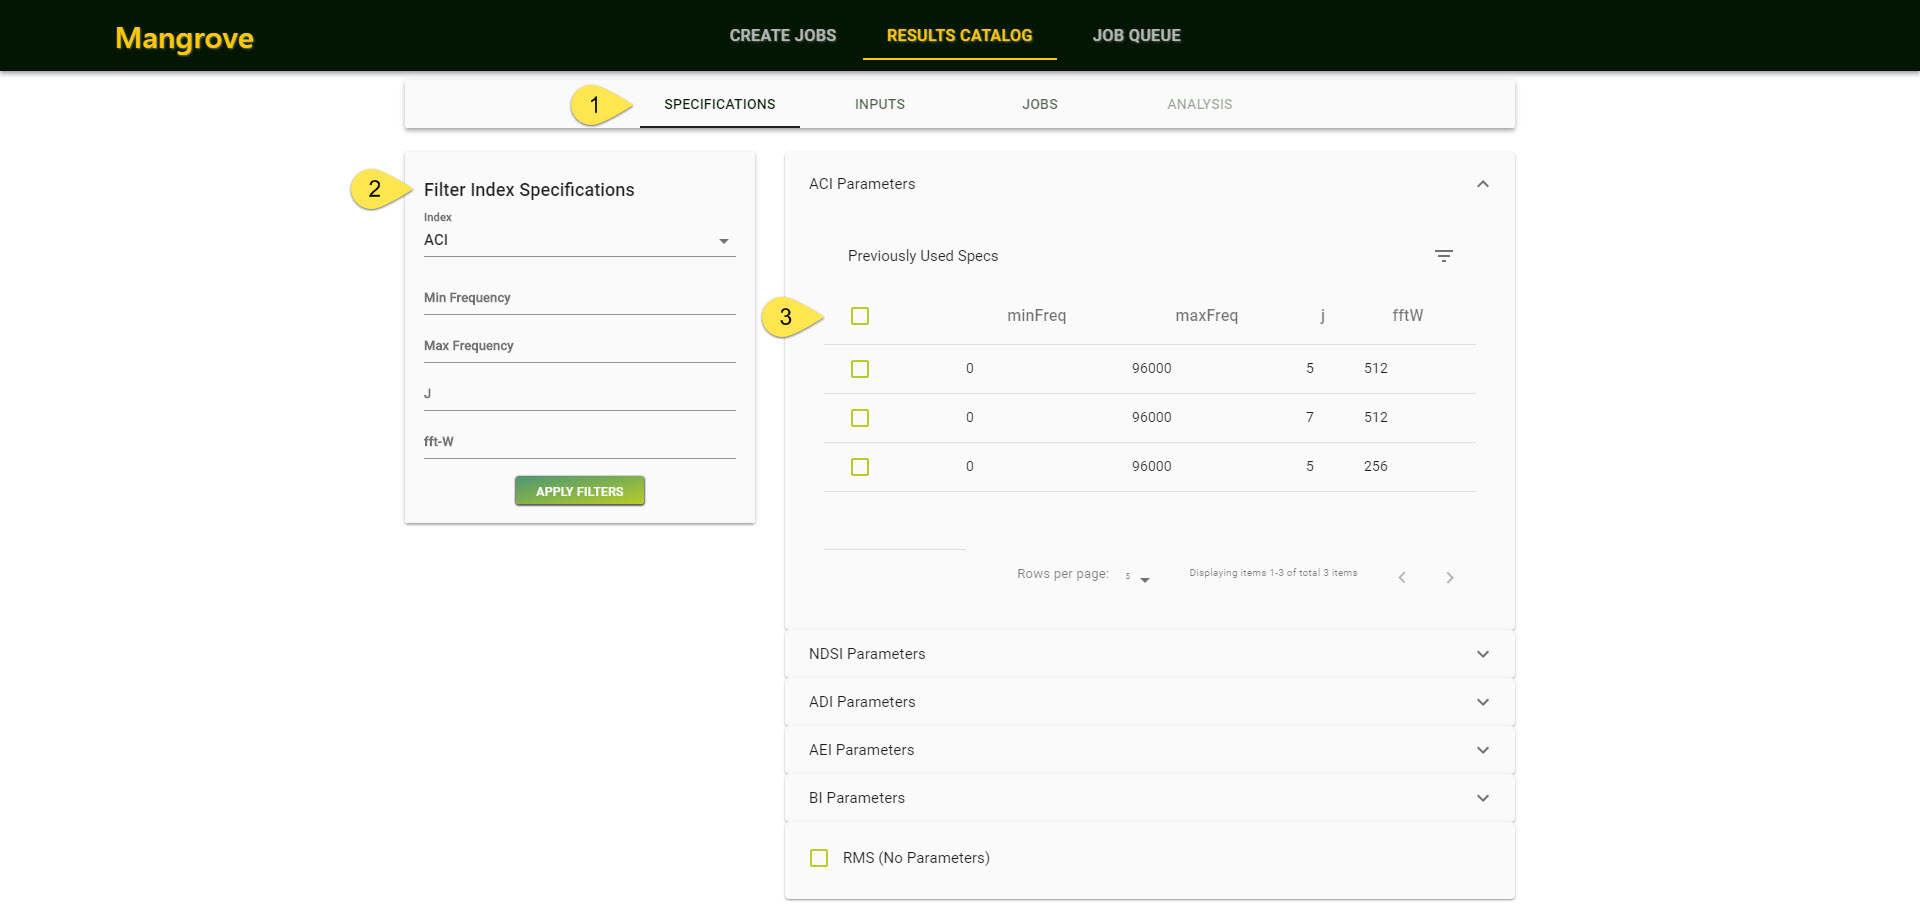
\includegraphics[width=\textwidth]{catalog-1}
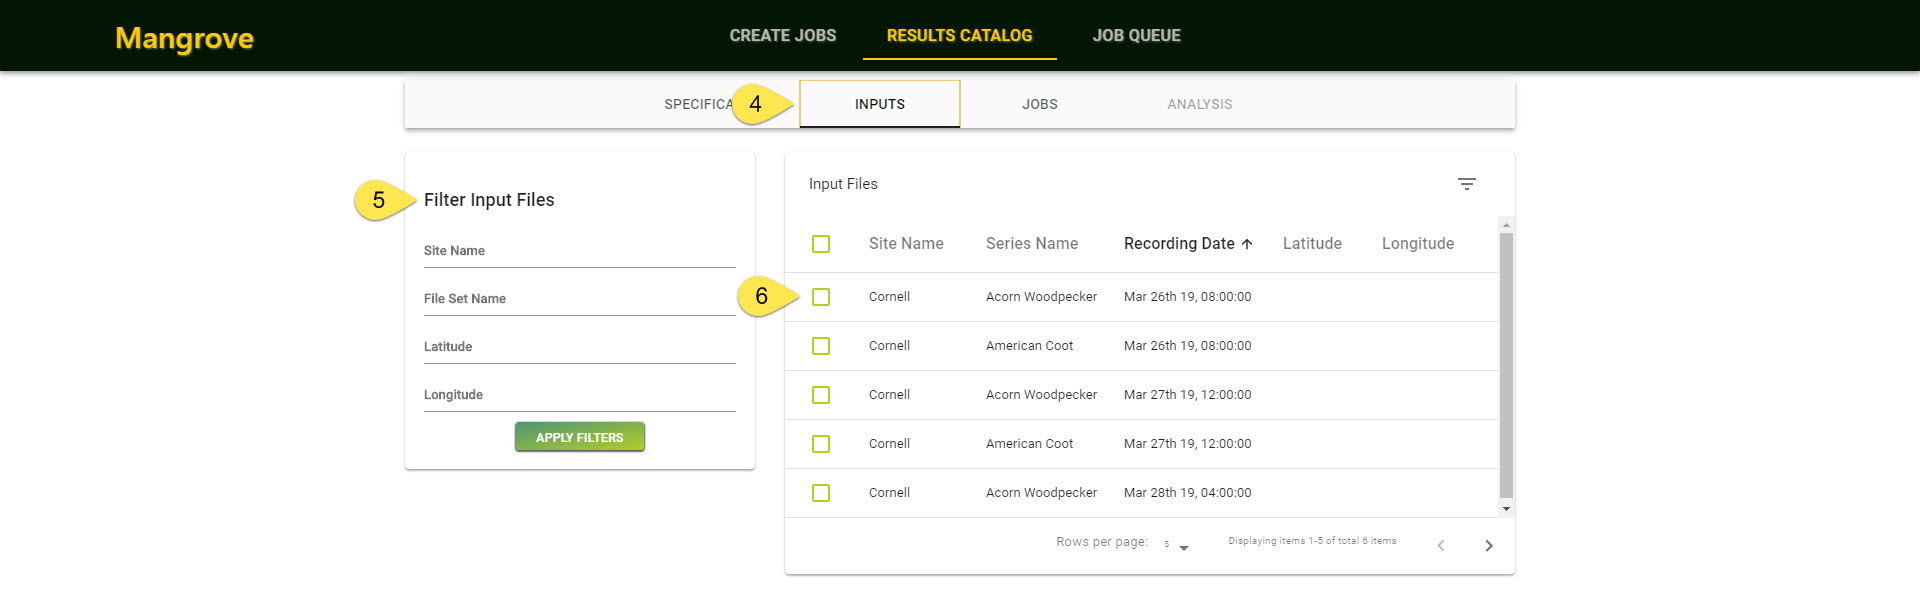
\includegraphics[width=\textwidth]{catalog-2}
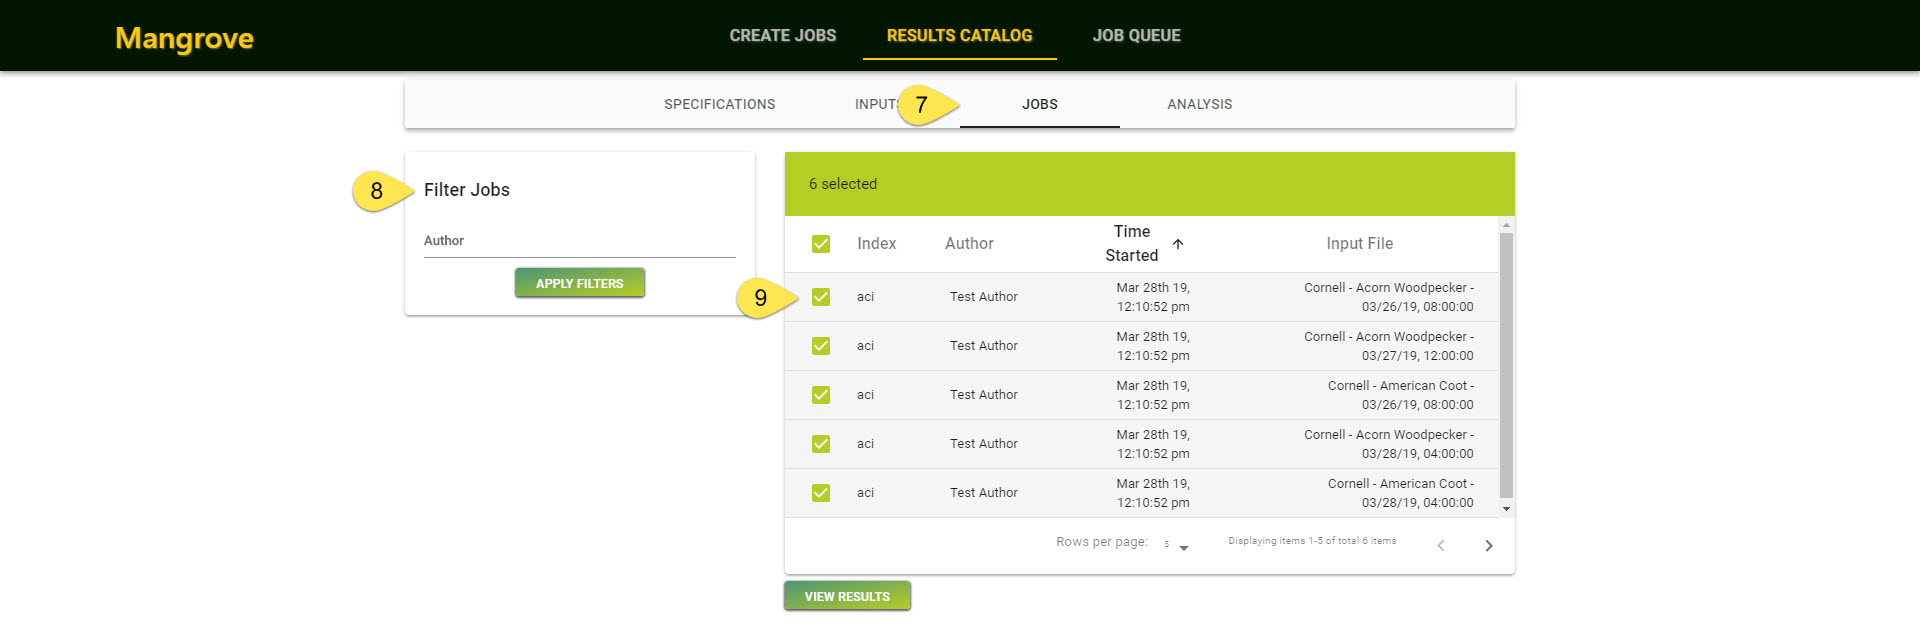
\includegraphics[width=\textwidth]{catalog-3}
\begin{enumerate}
    \item \textbf{Select Specifications}\\ First the user will select the specifications they wish to use to define the inputs and jobs they want to view results for.
    \item \textbf{Filter Specifications}\\ This section consists of a set of filter options for each index. Every index has different parameters, so the user can define a filter of those parameters to find the specs they wish to use. Combined with job searching, a user could view results of jobs on files taken in the same location, but analyzed with different indices.
    \item \textbf{Select Spec By Index}\\ For every available index, the defined specs will be listed. Multiple specs from different indices can be selected as well. The user will then select any spec they wish to use from any index using the checkboxes. Additionally, the user can sort any parameter.
    \item \textbf{Select Inputs}\\ After selecting specs, the next step is to select inputs that match the selected specs. Here, only inputs that have had jobs run on them with the selected specs will appear.
    \item \textbf{Filter By Metadata}\\ The user can filter the input files by its user defined metadata. When creating jobs, the user creates a Site and Series name for all inputs to be a part of. Here, they can type in a Site or Series to filter by. Additionally, they can filter by specific longitude and latitude markers.
    \item \textbf{Select Filtered Inputs}\\ After filtering, the user will select their inputs using the checkboxes. Again, these can be sorted by Site name, Series name, and also the date of the recording. An example of searching by Site, such as \textquotesingle UCF Arboretum\textquotesingle , would show all files captured at that location. An additional feature to this table is that you can delete inputs. Deleting inputs also removes any associated jobs with the input.
    \item \textbf{Select Jobs}\\ The final step before viewing graphs in the Analysis View is to choose jobs based off of the selected specs and inputs. As explained previously in this paper, every job consists of a spec and an input file. Thus, only jobs containing both selected specs and inputs will appear here.
    \item \textbf{Filter By Author}\\ The user can filter jobs by Author here. When on a shared server instance, other user\textquotesingle s jobs may be available to be viewed as long as the proper permissions are given.
    \item \textbf{Select Filtered Jobs}\\ Finally, the user can once again select jobs using the checkboxes provided. The user can also sort these jobs by author and also by the time in which the job was created.
\end{enumerate}
The second part of the Results Catalog is referred to as the Analysis View. The Analysis View focuses on having a clear way for users to view meaningful visualizations of their sound files and results. The features of the Analysis View are outlined below.\\
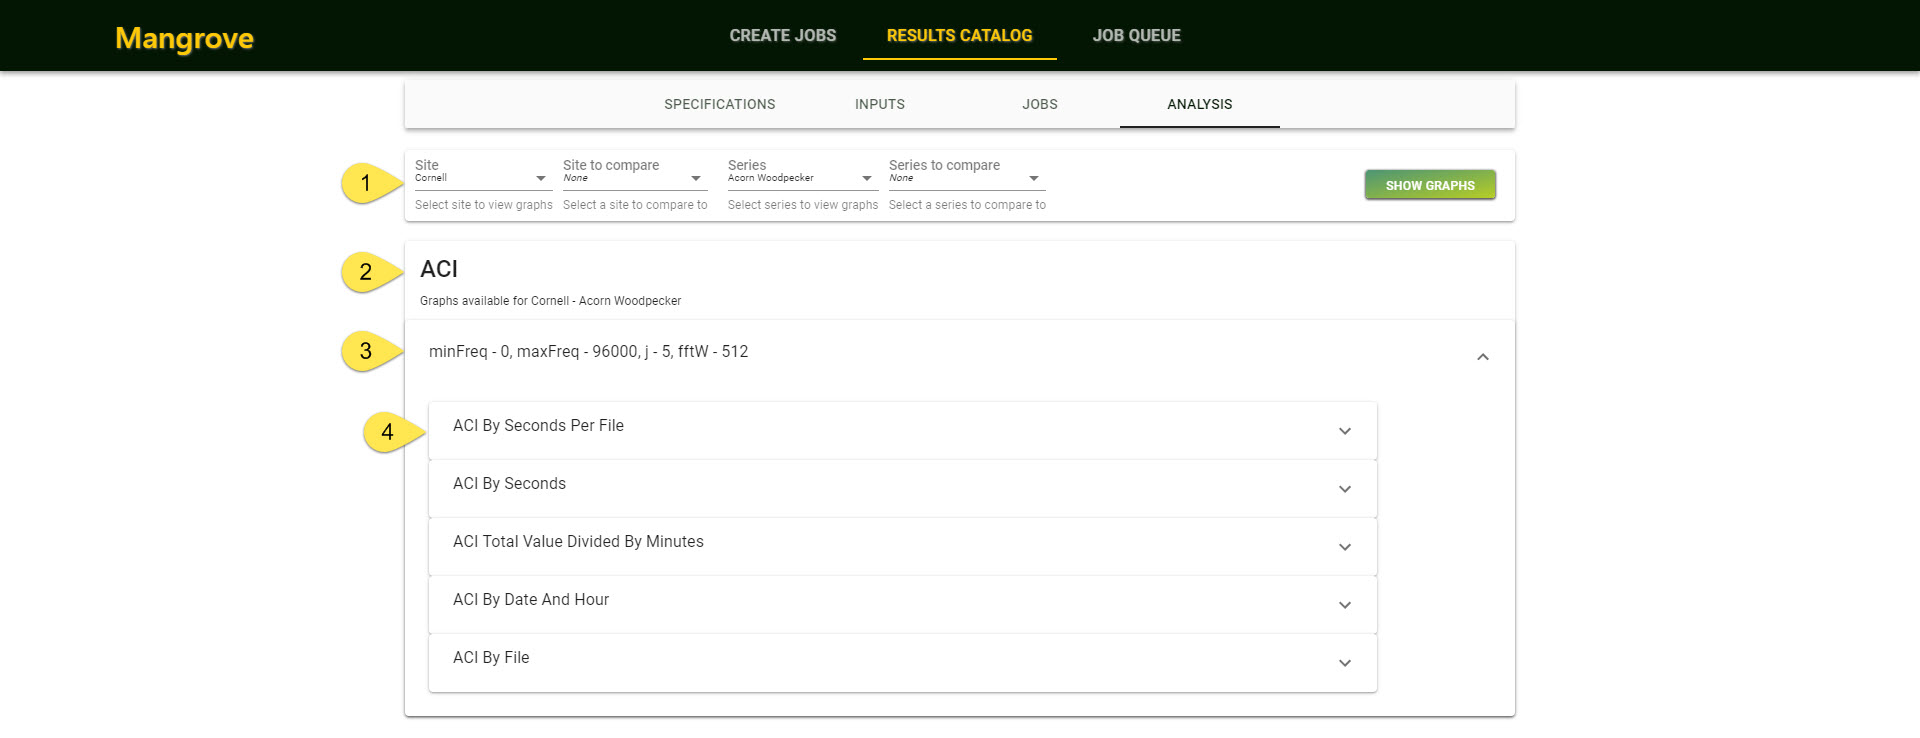
\includegraphics[width=\textwidth]{catalog-4}
\begin{enumerate}
  \item \textbf{Analysis View}\\ Before any graphs are shown in the Analysis View, the user must select which Site and Series they wish to view graphs for. If they wish, they can choose a Site and Series to compare to as well. When they have selected these, clicking the Show Graphs button will make the graphs appear.
  \item \textbf{Graphs Sorted By Index}\\ In the example shown, only the ACI index is available. However if the user selected another index, like NDSI, another panel like the ACI one will appear below the ACI one. This panel contains all the specs selected in the previous steps, along with the graphs for those specs. All of which are contained in drop down containers.
  \item \textbf{Graphs Sorted By Spec}\\ For each selected spec from the earlier steps, a drop down container will appear with the title description of the spec\textquotesingle s parameters.
  \item \textbf{Graphs}\\ These drop down containers contain the graphs themselves. Every index has different graphs available meant to best represent the index and its respective outputs. For most indices, any data point on the graphs can be clicked to bring up an audio player. This will automatically start playing the sound file at the timestamp corresponding to the point clicked. These graphs are detailed more in the Creating Flexible Data Visualizations section of this paper.
  \item \textbf{Export To CSV}\\ Along with viewing graphs, an option to export the results of jobs to a CSV file is available. The main purpose of this feature is to confirm the credibility of the visualizations, which is especially important in research publications.
\end{enumerate}
Clicking this button will open the modal shown below, where the user can specify certain preferences on how the data will be exported.\\
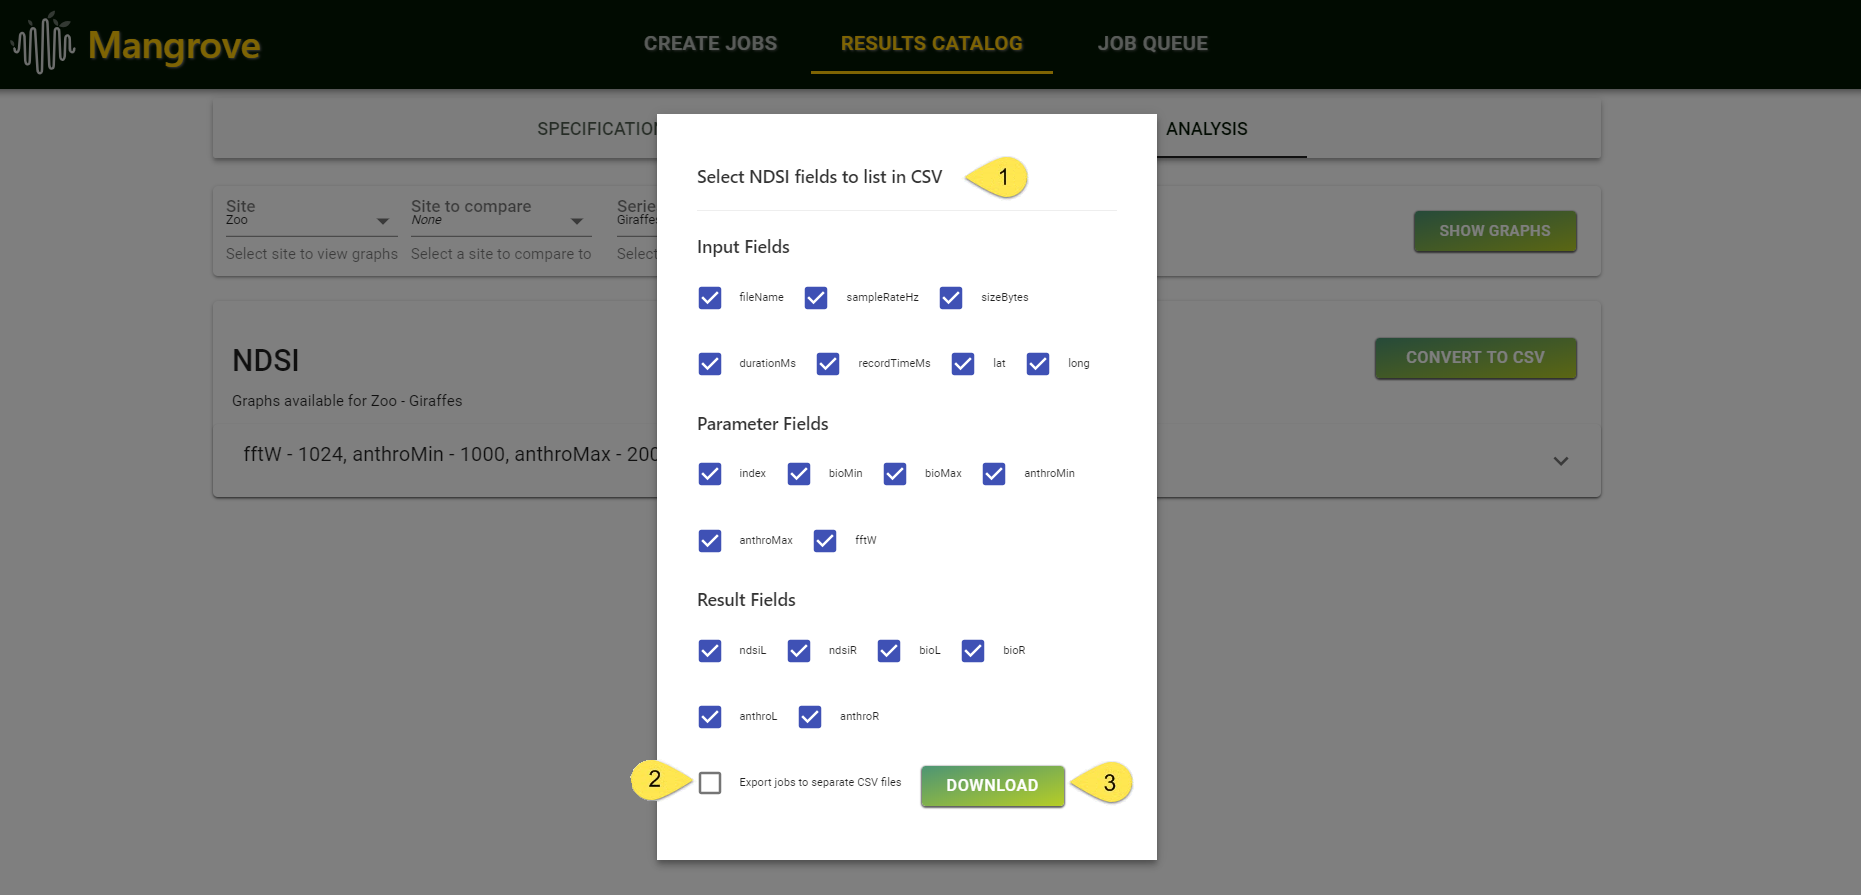
\includegraphics[width=\textwidth]{CSVExport}
\begin{enumerate}
  \item \textbf{Specify CSV Fields}\\ The user is shown check boxes of all parameters used to create this set of jobs as well as the name of each result value produced. If certain parameters or results are not relevant to the user\textquotesingle s current research, they can be omitted so that the important data is easier to read.
  \item \textbf{Export as Separate CSVs}\\ The default option is to produce a CSV file of the entire job set selected in the catalog. Some indices however, like ACI have very large array results, which take up multiple rows in the file. The option to convert each job as a separate file is given to make the results clearer to read.
  \item \textbf{Download}\\ When all fields and CSV type preferences have been specified, the user can download the job set CSV file or each individual file. When downloaded, job set files will be named according to the site, series and index used, while individual job files will be named with the site, series and filename.
\end{enumerate}
